\chapter{C 语言程序终止性的自动验证}
\label{cha:c-termination}

上一章从建模方法论的角度,试图提高规范化条件重写模型作为一种建模模型的易用性。本章将从另外一个角度切入,进一步降低利用规范化条件重写模型进行建模验证的成本。在此前的讨论中,建模过程不针对任何特定的验证属性。这要求建立的模型应尽可能涵盖系统各方面的行为特征,并包含尽可能多的细节,使得针对模型任何属性的验证结果都可以代表系统的性质。因此,为了保证模型与系统的等价性以及抽象程度的合理性,建模过程只能通过人工进行。然而,如果只针对某种特定属性,如可达性、终止性等,则建模过程只需要针对系统行为的某个侧面进行。这将显著地降低建模的难度,使得建模过程的自动化成为可能。

本章在已有对 C 语言程序自动建模的工作基础上,开发实现了针对 C 语言程序终止性的自动验证工具 \CTerm。

\section{引言}

程序的终止性问题是验证领域的一个重要问题。它的重要性主要体现在两个方面。首先,终止性是完全正确性(Total correctness)的必要条件。一个程序(或算法)被称作完全正确,当且仅当它是终止的,且它的行为符合其规约(Specification)的规定。用 Hoare 逻辑~\cite{DBLP:journals/cacm/Hoare69} 表示,三元组 $\{P\}~\texttt{C}~\{Q\}$ 成立,当且仅当在满足谓词 $P$ 的前提下,(i) 程序 $\texttt{C}$ 终止;且 (ii) 执行完 $\texttt{C}$ 后谓词 $Q$ 成立。而一个程序(或算法)称作部分正确,则只要求在假设它终止的前提下,其行为符合规约的规定。也就是说,三元组 $\{P\}~\texttt{C}~\{Q\}$ 成立,当且仅当在满足谓词 $P$ 的前提下,如果程序 \verb|C| 终止,则执行完 $\texttt{C}$ 后谓词 $Q$ 成立。举以下简单例子:
\begin{verbatim}
    {x == 1} while (true) x = x; {y == 2}
\end{verbatim}
由于其 \verb|while| 循环不终止,该程序根据其规约,不是完全正确的,但它是部分正确的。

程序终止性的第二个重要性在于,对 CTL~\cite{DBLP:conf/lop/ClarkeE81}、CTL*~\cite{DBLP:journals/jacm/EmersonH86}、Fair-CTL~\cite{DBLP:journals/jcss/EmersonH85} 以及 LTL~\cite{DBLP:conf/banff/Vardi95} 性质的验证,可以转化为对安全性~\cite{DBLP:journals/tse/Lamport77}(safety)和对终止性的验证~\cite{DBLP:conf/tacas/BrockschmidtCIK16}。由于目前大多数程序验证工具都针对安全性进行验证,因此终止性验证工具的研究理论上可以提升这些程序验证工具的验证能力。

嵌入式系统的软件部分通常由 C 语言进行实现,因此开发 C 语言程序的终止性自动验证工具,对保障嵌入式系统的可靠性具有重要意义。

程序的终止与否,有时候并不容易判断,如以下例子(Collatz 问题):
\begin{verbatim}
    while (x > 1) {
      if (even(x))  x = x / 2;
      else  x = 3 * x + 1;
    }
\end{verbatim}
目前有许多技术可以自动验证一个程序的终止性,而其中一种主流技术正是基于整数重写模型~\cite{DBLP:conf/rta/FalkeKS11}。整数重写模型可以看作是规范化条件重写模型的一种特例。在第~\ref{cha:normalrewriting} 章已经提到,重写模型的终止性是该领域的最重要问题之一,目前已经有大量关于重写模型终止性的验证理论及工具。通过将程序(自动)建模成整数重写模型,程序终止性问题就可以被转化为重写模型的终止性问题,从而使用对应的技术进行解决。本文基于这种技术路线,开发了 C 语言程序终止性自动验证工具 \CTerm。

本章其余部分组织结构如下:第~\ref{s:termination-related} 小节介绍相关的 C 程序终止性自动验证工具;第~\ref{s:termination-models} 小节讨论如何自动建立 C 程序的整数重写模型,以便对程序终止性进行验证;\CTerm 工具将在第~\ref{s:ceagle-termination} 小节进行介绍;最后对本章内容进行简要小结。 

\section{相关工作}
\label{s:termination-related}

对指令式程序的终止性进行自动验证,目前主要有三种主流技术。 

排序函数~\cite{DBLP:conf/lics/PodelskiR04}(ranking function)是最经典的用于证明程序终止性的技术。排序函数 $rank$ 将每一个程序状态 $s$ 映射为抽象域(如正整数域)中的一个元素 $rank(s)$。如果对于程序的每一步执行 $s \ra s'$,排序函数满足 $rank(s) > rank(s')$,且抽象域上的二元关系 $>$ 是良基的(Well-founded),即不存在无穷递减序列,则该程序是终止的。于是验证程序终止性的问题可以被归约为排序函数的构造问题。如果满足条件的排序函数存在,则可判断该程序终止。基于排序函数构造的自动验证工具主要有 \textsc{OctaTerm}~\cite{DBLP:conf/popl/BerdineCCDO07}、\textsc{PolyTerm}~\cite{DBLP:conf/popl/BerdineCCDO07}、FuncTion~\cite{DBLP:conf/sas/Urban13,DBLP:conf/tacas/Urban15} 和 \textsc{c2fsm+Aspic+Rank}~\cite{DBLP:conf/sas/AliasDFG10}。其中 \textsc{OctaTerm} 和 \textsc{PolyTerm} 并不支持 C 程序的输入,而 FuncTion 和 \textsc{c2fsm+Aspic+Rank} 可以支持。

针对排序函数构造困难的问题,ARMC~\cite{DBLP:conf/padl/PodelskiR07}、CProver~\cite{DBLP:conf/cav/KroeningSTW10,DBLP:conf/tacas/TsitovichSWK11}、TERMINATOR~\cite{DBLP:conf/pldi/CookPR06} 及其后继工具 T2~\cite{DBLP:conf/tacas/BrockschmidtCIK16} 等 C 程序终止性验证工具采用了递增式的排序函数构造技术。这些工具将安全性检查过程集成到排序函数的构造过程中。其主要原理是,若当前已经有排序函数 $rank$ 对程序的某些执行序列满足递减关系,则利用安全性检查工具找到一条不能使 $rank$ 递减的执行序列 $\pi$;根据反例 $\pi$ 对 $rank$ 进行改善,得到新的排序函数 $rank'$。重复此过程直到构造的排序函数能使程序的所有执行序列满足递减关系。同样基于排序函数结合安全性检查技术的 C 程序终止性验证工具还有 \textsc{SeaHorn}~\cite{DBLP:conf/tacas/UrbanGK16} 和 2LS~\cite{DBLP:conf/kbse/ChenDKSW15}。在 \textsc{SeaHorn} 的实现中,安全性检查技术的使用方式与其它工具稍有不同,目的是为了在对当前排序函数进行改善时,能获得更多信息。而 2LS 则将过程间分析技术加入到排序函数的构造过程中。 
 
另一个主流技术是将程序的终止性验证问题归约为重写模型的终止性判定问题。通过利用重写模型(或其扩展形式)对程序中影响终止性的行为进行自动建模,若模型具有终止性,则可判定该程序也具有终止性。这种技术方案的好处是可以充分利用重写领域对终止性的判定技术,如递归路径序~\cite{DBLP:journals/jsc/Dershowitz87}(Recursive path order)、Knuth-Bendix 序~\cite{knuth1983simple}(Knuth-Bendix order)、依赖对~\cite{DBLP:journals/tcs/ArtsG00,DBLP:journals/jsc/GieslAO02}(Dependency pair)等。基于这种技术方案的 C 程序终止性验证工具主要有 AProVE~\cite{DBLP:conf/cade/GieslBEFFOPSSST14}、\verb|llvm2KITTeL|+\verb|KITTeL|~\cite{DBLP:conf/rta/FalkeKS11}(以下简称为 \verb|KITTeL|) 和 c2lctrs+Ctrl~\cite{DBLP:conf/lpar/Kop015,KN15}(以下简称为 Ctrl)。其中 \verb|KITTeL| 和 Ctrl 的模型直接从 C 程序的控制流图中进行抽取,因此无法对涉及指针的程序行为进行描述。而 AProVE 先通过符号执行技术构造程序的一种中间表示形式——符号执行图(Symbolic execution graph),然后再从中抽取重写模型。由于符号执行图包含了程序中涉及指针的行为,因此 AProVE 的技术方案能更好地处理包含内存操作的 C 程序。

近年来也出现了一些新兴的技术可用于验证 C 程序的终止性。例如工具 HipTNT+~\cite{DBLP:conf/pldi/LeQC15} 实现了一种基于函数摘要(Summary)的终止性验证技术,通过推理得到每个函数的终止性或非终止性的摘要,然后综合得到整个程序的终止性验证结果。Ultimate B\"uchi Automizer~\cite{DBLP:conf/cav/HeizmannHP14} 实现了一种基于程序构造的终止性验证技术。它首先对程序进行执行路径采样,得到若干套索形状(Lasso-shaped)的程序执行路径;然后根据这些路径构造出若干具有终止性的程序片段;重复该过程直到构造出来的程序片段集合可以涵盖目标程序的行为,则终止性得到证明。

本文开发的 C 程序终止性自动验证工具 \CTerm 采用基于重写模型的验证技术,且利用符号执行图作为程序的中间表示形式,与 AProVE 工具类似。AProVE 作为一个闭源工具,其实现细节我们不得而知,但根据文献~\inlinecite{DBLP:journals/jar/StroderGBFFHSA17} 的描述,AProVE 的符号执行图构造过程在遇到递归函数时,可能无法终止。   \CTerm 与 AProVE 的主要区别在于,\CTerm 采用了单函数的内存模型,保证了符号执行图的构造过程在遇到递归函数时可以终止。


\section{C 程序的整数重写模型}
\label{s:termination-models}

对 C 程序的终止性进行自动验证,其关键在于自动化构建 C 程序对应的整数重写模型。本文采取文献~\inlinecite{DBLP:conf/cade/StroderGBFFHS14} 的方法,基于符号执行技术构建 C 程序的符号执行图,再从符号执行图生成适用于终止性验证的整数重写模型。

\begin{figure}[ht]
\centering
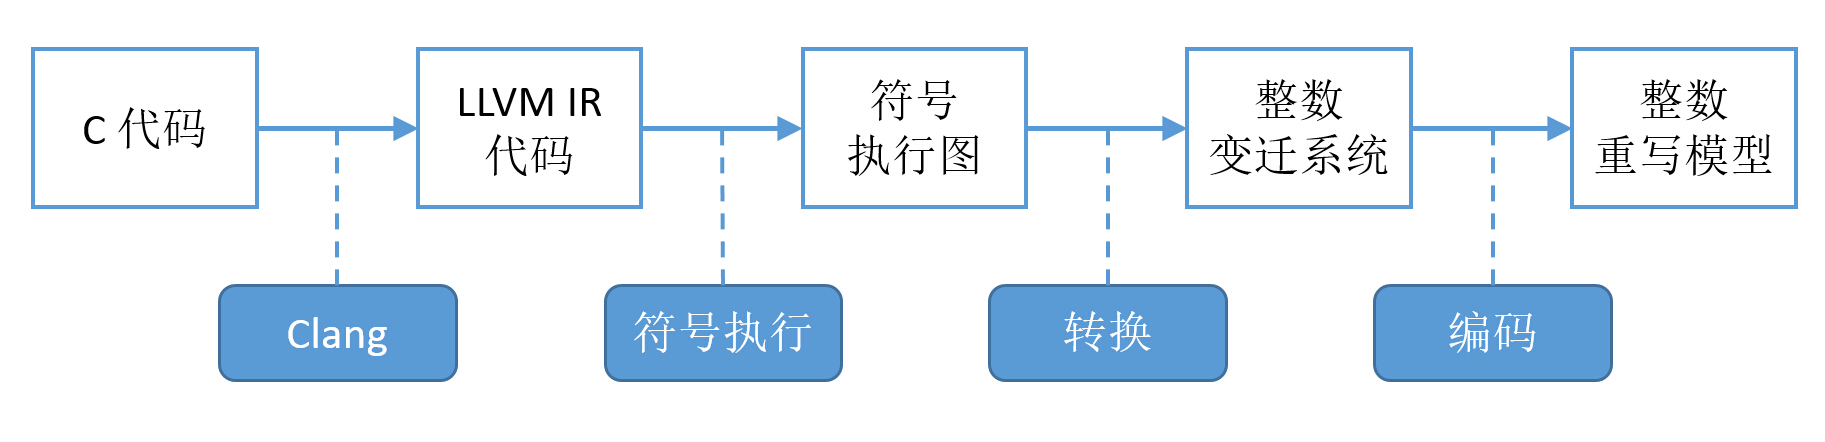
\includegraphics[width=\textwidth]{C2intTRS.jpg}
\caption{C 程序的整数重写模型自动构造}
\label{f:C2intTRS}
\end{figure}

图~\ref{f:C2intTRS} 是 C 程序的整数重写模型自动构造流程。C 程序经过编译器 Clang 的编译后生成对应的 LLVM IR~\cite{DBLP:conf/cgo/LattnerA04} 代码。基于这些 LLVM IR 代码,利用符号执行技术~\cite{DBLP:journals/cacm/King76},产生输入程序的符号执行图~\cite{DBLP:conf/lopstr/GieslSSEF12}。整数变迁系统~\cite{DBLP:journals/cacm/Keller76} 描述了该符号执行图的终止性行为。最后利用重写模型丰富的表达能力,将该整数变迁系统的语义编码成整数重写模型的形式。

这个构造过程涉及到三个重要的模型:符号执行图、整数变迁系统和整数重写模型。在本小节接下来的部分将对这三个概念进行介绍,并对其构造的核心原理进行描述。

\subsection{符号执行图}
\label{ss:seg}

\emph{符号执行图}(Symbolic execution graph)是由 Giesl 等人提出的用于描述程序执行过程的数据结构~\cite{DBLP:conf/lopstr/GieslSSEF12}。一个符号执行图是一个有向图,它包含一个顶点集合和一个边集合。每个顶点代表一个\emph{抽象}的程序执行状态,它包含程序当时的位置(pc)、变量赋值状态、内存分配情况等信息。程序执行图的边分为三类:
\begin{enumerate} [(i)]
\item 求值(Evaluation)类型。求值类型的边表示:若其起始顶点表示的程序状态为 $s$,当前程序位置为 $p$($p$ 也是状态 $s$ 中包含的信息),则 $s$ 在执行 $p$ 位置的程序指令后,其状态 $s'$ 为该有向边的终止顶点代表的状态。
\item 精化(Refinement)类型。精化类型的边的终止顶点 $v$ 所表示的状态是起始顶点 $u$ 表示的状态的精化,即 $v$ 所表示的程序状态集合是 $u$ 所表示的程序状态集合的子集。
\item 抽象(Abstraction)类型。抽象类型的边与精化类型的边相反,它表示其终止顶点 $v$ 的状态是起始顶点 $u$ 状态的抽象,即 $u$ 所表示的程序状态集合是 $v$ 所表示的程序状态集合的子集。
\end{enumerate}

至于每个顶点所表示的抽象程序状态,本文基于文献~\inlinecite{DBLP:conf/cade/StroderGBFFHS14} 的定义,进行了简化:
\begin{definition}[抽象程序状态] 
\label{d:abstract-state}
给定程序变量集合 $\VP$,符号化变量集合 $\Vsym$,程序位置集合 $Pos$,则一个抽象程序状态是一个六元组 $\lb p, LV, LAL, KB, AL, PT \rb$。其中 $p\in Pos$;$LV : \VP \ra \Vsym$;$LAL = \{\interp{v_1,v_2}\mid v_1,v_2\in\Vsym, v_1\le v_2 \}$;$KB\subseteq QF\_IA(\Vsym)$;$AL = \{\interp{v_1,v_2}\mid v_1,v_2\in\Vsym, v_1\le v_2 \}$;$PT \subseteq \{(v_1\pta_{\ty} v_2)\mid v_1,v_2\in\Vsym, \ty \mbox{是LLVM的类型}\}$。另外,抽象程序状态 $ERR$ 表示可能违背了内存安全的状态;抽象程序状态 $END$ 表示执行结束的程序状态。
\end{definition}

直观上解释,$LV$(Local variables)表示该状态的程序变量赋值情况,程序变量值由集合 $\Vsym$ 中的符号化变量表示;$LAL$(Local allocation list)表示局部内存分配情况,二元组 $\interp{v_1,v_2}$ 表示在 $v_1$ 和 $v_2$ 之间的内存单元是已经过分配的;$QF\_IA(\Vsym)$ 是指\emph{无量词的}(Quantifier-free)一阶公式,用于描述 $\Vsym$ 变量的\emph{整数代数}(Integer arithmetic)性质,$KB$(Knowledge base)是该状态满足的性质集合;$AL$(Allocation list)与 $LAL$ 类似,表示的是全局内存分配情况;$PT$(Pointer table)表示内存状态,元组 $(v_1\pta v_2)$ 表示内存地址 $v_1$ 指向的内容是 $v_2$,具有类型 $\ty$。

定义~\ref{d:abstract-state} 与文献~\inlinecite{DBLP:conf/cade/StroderGBFFHS14} 对抽象程序状态定义的最主要区别是,定义~\ref{d:abstract-state} 描述了单函数的抽象状态,而文献~\inlinecite{DBLP:conf/cade/StroderGBFFHS14} 的定义包含了栈结构,允许描述多函数之间的调用。

基于我们的简化定义,我们定义用于描述每个抽象程序状态的一阶谓词集合 $\lb a\rb$:
\begin{definition}[\inlinecite{DBLP:journals/jar/StroderGBFFHSA17}]
给定抽象程序状态 $a$,一阶谓词集合 $\lb a\rb$ 是满足以下条件的最小集合:
\begin{eqnarray}
\lb a \rb & = & KB 
\cup \{1\le v_1\land v_1\le v_2 
    \mid \interp{v_1, v_2} \in LAL \cup AL  \} \nonumber \\
& & \cup\; \{ v_2 < w_1 \lor w_2 < v_1 
    \mid \interp{v_1,v_2},\interp{w_1,w_2}\in LAL\cup AL, (v_1,v_2)\not= (w_1,w_2) \}    \nonumber \\
& & \cup\; \{ v_2 = w_2 \mid (v_1\pta_{\ty}v_2),(w_1\pta_{\ty}w_2)\in PT 
    \mbox{ and } \vDash \lb a\rb \Dra  v_1=w_1   \} \nonumber \\
& & \cup\; \{ v_1 \not= w_1 \mid (v_1\pta_{\ty}v_2),(w_1\pta_{\ty}w_2)\in PT 
    \mbox{ and } \vDash \lb a\rb \Dra  v_2\not=w_2   \} \nonumber \\
& & \cup\; \{ v_1 > 0 \mid (v_1\pta_{\ty} v_2) \in PT \} \;\;\mbox{。} \nonumber
\end{eqnarray}
\end{definition}

需要注意,$\lb a\rb$ 是归纳定义的。$\lb a \rb$ 定义了抽象程序状态 $a$ 满足的一阶谓词性质集合。

符号执行图的构建基于符号执行规则进行。给定一个抽象程序状态,根据符号执行规则计算下一个(或两个)抽象程序状态。由于实际的程序状态空间可能是无穷的,为了用符号执行图的有穷顶点数表示无穷的程序状态空间,在构造过程中需要根据一定的策略对抽象程序状态进行抽象。下面先介绍符号执行规则,再介绍符号执行图的构造策略。

基于定义~\ref{d:abstract-state},我们对文献~\inlinecite{DBLP:conf/cade/StroderGBFFHS14} 和~\inlinecite{DBLP:journals/jar/StroderGBFFHSA17} 的符号执行规则进行简化。以下列举其中较关键的几条符号执行规则。


\begin{table}[htbp]
\caption{符号执行规则:\texttt{load} 指令(内存已分配)}
\label{tab:rule-load-alloc}
\begin{tabularx}{\textwidth}{|X|}
\hline
\textbf{\texttt{load}} \emph{已分配内存} \\
{\centering $
\inferrule
   {\lb p, LV, LAL, KB, AL, PT\rb}
   {\lb p^+, LV[\texttt{x}:= w], LAL, KB, AL, PT\cup\{LV(\texttt{ad})\pta_{\ty} w \}\rb }
$ \\}
\textbf{如果满足以下条件} \\
~$\bullet$ $p$ : "\texttt{x = load ty* ad}" 其中 $\texttt{x},\texttt{ad}\in\VP$; \\
~$\bullet$ 存在 $\interp{v_1,v_2}\in LAL\cup AL$ \newline 
~\phantom{$\bullet$ } 使得 $\vDash \lb a\rb \Dra (v_1\le LV(\texttt{ad}) \land LV(\texttt{ad}) + size(\ty)-1\le v_2)$;  \\
~$\bullet$ $w\in\Vsym$ 是新变量。 \\
\hline
\end{tabularx}
\end{table}

\begin{table}[htbp]
\caption{符号执行规则:\texttt{load} 指令(内存未分配)}
\label{tab:rule-load-unalloc}
\begin{tabularx}{\textwidth}{|X|}
\hline
\textbf{\texttt{load}} \emph{未分配内存} \\
{\centering $
\inferrule
   {\lb p, LV, LAL, KB, AL, PT\rb}
   {ERR}
$ \\}
\textbf{如果满足以下条件} \\
~$\bullet$ $p$ : "\texttt{x = load ty* ad}" 其中 $\texttt{x},\texttt{ad}\in\VP$; \\
~$\bullet$ 不存在 $\interp{v_1,v_2}\in LAL\cup AL$ \newline 
~\phantom{$\bullet$ } 使得 $\vDash \lb a\rb \Dra (v_1\le LV(\texttt{ad}) \land LV(\texttt{ad}) + size(\ty)-1\le v_2)$。  \\
\hline
\end{tabularx}
\end{table}

表~\ref{tab:rule-load-alloc} 和~\ref{tab:rule-load-unalloc} 分别是 \verb|load| 指令从已分配内存和未分配内存中读取数据时对应的符号执行规则。如表~\ref{tab:rule-load-alloc} 所示,当 \verb|load| 指令准备从地址 \verb|ad| 中读取数据时,需要先判断是否能根据当前抽象程序状态 $a$ 的谓词表达式 $\lb a \rb$ 推断出地址 \verb|ad| 对应的内存块 $\interp{LV(\texttt{ad}), LV(\texttt{ad})+ size(\ty) -1}$ 已经经过分配。如果该内存块已经经过分配,则可执行表~\ref{tab:rule-load-alloc} 中的符号执行规则生成新的抽象程序状态,新状态中的程序变量 \verb|x| 得到更新,程序指针指向 $p$ 的下一条指令 $p^+$。如果不能推断出该内存块已经经过分配,则如表~\ref{tab:rule-load-unalloc} 所示,将产生抽象程序状态 $ERR$。

\begin{table}[htbp]
\caption{符号执行规则:\texttt{icmp eq} 指令(命题成立)}
\label{tab:rule-icmp-eq-true}
\begin{tabularx}{\textwidth}{|X|}
\hline
\textbf{\texttt{icmp eq}} \emph{命题为真} \\
{\centering $
\inferrule
   {\lb p, LV, LAL, KB, AL, PT\rb}
   {\lb p^+, LV[\texttt{x} := w], LAL, KB\cup\{w=1\}, AL, PT\rb}
$ \\}
\textbf{如果满足以下条件} \\
~$\bullet$ $p$ : "\texttt{x = icmp eq ty $t_1$, $t_2$}" 其中 $\texttt{x}\in\VP$ 且 $t_1,t_2\in\VP\cup\mathbb{Z}$; \\
~$\bullet$ $\vDash \lb a\rb \Dra (LV(t_1) = LV(t_2))$;  \\
~$\bullet$ $w\in\Vsym$ 是新变量。 \\
\hline
\end{tabularx}
\end{table}

\begin{table}[htbp]
\caption{符号执行规则:\texttt{icmp eq} 指令(命题不成立)}
\label{tab:rule-icmp-eq-false}
\begin{tabularx}{\textwidth}{|X|}
\hline
\textbf{\texttt{icmp eq}} \emph{命题为假} \\
{\centering $
\inferrule
   {\lb p, LV, LAL, KB, AL, PT\rb}
   {\lb p^+, LV[\texttt{x} := w], LAL, KB\cup\{w=0\}, AL, PT\rb}
$ \\}
\textbf{如果满足以下条件} \\
~$\bullet$ $p$ : "\texttt{x = icmp eq ty $t_1$, $t_2$}" 其中 $\texttt{x}\in\VP$ 且 $t_1,t_2\in\VP\cup\mathbb{Z}$; \\
~$\bullet$ $\vDash \lb a\rb \Dra (LV(t_1) \not= LV(t_2))$;  \\
~$\bullet$ $w\in\Vsym$ 是新变量。 \\
\hline
\end{tabularx}
\end{table}

表~\ref{tab:rule-icmp-eq-true} 和~\ref{tab:rule-icmp-eq-false} 是指令 \verb|icmp| 的符号执行规则。这里只列出了 \verb|icmp eq| 的具体规则,其它比较操作(如 \verb|ule|、\verb|uge| 等)的规则类似。如果当前状态的性质集合 $\lb a\rb$ 可以推断出 \verb|icmp eq| 指令对应命题为真,如表~\ref{tab:rule-icmp-eq-true} 所示,则下一状态将程序变量 \verb|x| 的值赋为 $w$,$KB$ 告诉我们 $w=1$。否则,如果 $\lb a\rb$ 足以推断出该命题为假,则 \verb|x| 对应的值为 0。
如果 $\lb a\rb$ 所包含的信息不能推断出目标命题的真假,这说明下一个状态需要分情况讨论。于是我们需要往当前的抽象程序状态加入更多的信息,对状态进行“精化”。

\begin{table}[htbp]
\caption{符号执行规则:精化(\texttt{icmp eq} 指令)}
\label{tab:rule-refine-icmp-eq}
\begin{tabularx}{\textwidth}{|X|}
\hline
\emph{对} \textbf{\texttt{icmp eq}} \emph{进行精化}  \\
{\centering $
\inferrule
   {\lb p, LV, LAL, KB, AL, PT\rb}
   {\lb p, LV, LAL, KB\cup\{\varphi\}, AL, PT\rb \;\;\mid\;\; \lb p, LV, LAL, KB\cup\{\lnot\varphi\}, AL, PT\rb}
$ \\}
\textbf{如果满足以下条件} \\
~$\bullet$ $p$ : "\texttt{x = icmp eq ty $t_1$, $t_2$}" 其中 $\texttt{x}\in\VP$ 且 $t_1,t_2\in\VP\cup\mathbb{Z}$; \\
~$\bullet$ $\not\vDash \lb a\rb \Dra \varphi$ 且 $\not\vDash \lb a\rb \Dra \lnot\varphi$; \\
~$\bullet$ $\varphi$ 是 $LV(t_1) \not= LV(t_2)$。 \\
\hline
\end{tabularx}
\end{table}

表~\ref{tab:rule-refine-icmp-eq} 是对指令 \verb|icmp eq| 进行精化的规则。若根据当前抽象状态的信息不能推断出命题 $\varphi$ 的真假,则精化规则产生两个新的抽象程序状态,两个状态的集合 $KB$ 分别加入了 $\varphi$ 的真假信息,使后续的状态求值可以继续进行。其它涉及条件比较的指令的精化规则,也可以类似地进行定义。

\begin{table}[htbp]
\caption{符号执行规则:\texttt{add} 指令}
\label{tab:rule-add}
\begin{tabularx}{\textwidth}{|X|}
\hline
\textbf{\texttt{add}} \\
{\centering $
\inferrule
   {\lb p, LV, LAL, KB, AL, PT\rb}
   {\lb p^+, LV[\texttt{x} := w], LAL, KB\cup\{w= LV(t_1) + LV(t_2)\}, AL, PT\rb} 
$ \\}
\textbf{如果满足以下条件} \\
~$\bullet$ $p$ : "\texttt{x = add ty $t_1$, $t_2$}" 其中 $\texttt{x}\in\VP$ 且 $t_1,t_2\in\VP\cup\mathbb{Z}$; \\
~$\bullet$ $w\in\Vsym$ 是新变量。 \\
\hline
\end{tabularx}
\end{table}

表~\ref{tab:rule-add} 展示了代数运算指令 \verb|add| 的符号执行规则。

\begin{table}[htbp]
\caption{符号执行规则:\texttt{alloca} 指令(分配错误)}
\label{tab:rule-alloca-err}
\begin{tabularx}{\textwidth}{|X|}
\hline
\textbf{\texttt{alloca}} \emph{失败} \\
{\centering $
\inferrule
   {\lb p, LV, LAL, KB, AL, PT\rb}
   {ERR} 
$ \\}
\textbf{如果满足以下条件} \\
~$\bullet$ $p$ : "\texttt{x = alloca ty, i$n$ $t$}" 其中 $\texttt{x}\in\VP$ 且 $t\in\VP\cup\mathbb{Z}$; \\
~$\bullet$ $\not\vDash \lb a\rb \Dra (LV(t) > 0)$。 \\
\hline
\end{tabularx}
\end{table}

\begin{table}[htbp]
\caption{符号执行规则:\texttt{alloca} 指令(分配成功)}
\label{tab:rule-alloca}
\begin{tabularx}{\textwidth}{|X|}
\hline
\textbf{\texttt{alloca}} \emph{成功} \\
{\centering $
\inferrule
   {\lb p, LV, LAL, KB, AL, PT\rb}
   {\lb p^+, LV[\texttt{x} := v_1], LAL\cup\{\interp{v_1,v_2}\}, KB\cup\{v_2= v_1 + size(\ty)\cdot LV(t)-1\}, AL, PT\rb} 
$ \\}
\textbf{如果满足以下条件} \\
~$\bullet$ $p$ : "\texttt{x = alloca ty, i$n$ $t$}" 其中 $\texttt{x}\in\VP$ 且 $t\in\VP\cup\mathbb{Z}$; \\
~$\bullet$ $\vDash \lb a\rb \Dra (LV(t) > 0)$; \\
~$\bullet$ $v_1,v_2\in\Vsym$ 是新变量。 \\
\hline
\end{tabularx}
\end{table}

表~\ref{tab:rule-alloca-err} 和~\ref{tab:rule-alloca} 是 \verb|alloca| 指令的符号执行规则。分配内存成功的前提是,当前状态信息足以推断出分配的内存块大小为正数,否则则产生错误状态 $ERR$(如表~\ref{tab:rule-alloca-err})。当分配内存成功时,新状态的主要变化是其局部内存分配表 $LAL$ 中增加了一块新的内存区域 $\interp{v_1,v_2}$。符号变量 $v_1$ 与 $v_2$ 的关系在性质集合 $KB$ 中体现。


\begin{table}[htbp]
\caption{符号执行规则:\texttt{call} 指令}
\label{tab:rule-call}
\begin{tabularx}{\textwidth}{|X|}
\hline
\textbf{\texttt{call}} \\
{\centering $
\inferrule
   {\lb p, LV, LAL, KB, AL, PT\rb}
   {\lb p^+, LV[\texttt{x} := w], LAL, KB, AL, PT\rb} 
$ \\}
\textbf{如果满足以下条件} \\
~$\bullet$ $p$ : "\texttt{x = call ty $\ldots$}" 其中 $\texttt{x}\in\VP$;\\
~$\bullet$ $w\in\Vsym$ 是新变量。 \\
\hline
\end{tabularx}
\end{table}

\begin{table}[htbp]
\caption{符号执行规则:\texttt{ret} 指令}
\label{tab:rule-ret}
\begin{tabularx}{\textwidth}{|X|}
\hline
\textbf{\texttt{ret}} \\
{\centering $
\inferrule
   {\lb p, LV, LAL, KB, AL, PT\rb}
   {END}
$ \\}
\textbf{如果满足以下条件} \\
~$\bullet$ $p$ : "\texttt{ret ty $t$}" 其中 $t\in\VP\cup\mathbb{Z}$。\\
\hline
\end{tabularx}
\end{table}

表~\ref{tab:rule-call} 和~\ref{tab:rule-ret} 分别是 \verb|call| 指令和 \verb|ret| 指令的符号执行规则。由于本文采用单函数分析的方法,因此对 \verb|call| 指令与 \verb|ret| 指令的处理比文献~\inlinecite{DBLP:conf/cade/StroderGBFFHS14} 和~\inlinecite{DBLP:journals/jar/StroderGBFFHSA17} 精简。应用 \verb|call| 指令时,由于我们对所有函数逐一进行终止性分析,因此可以假设被 \verb|call| 调用的函数将返回某值。于是表~\ref{tab:rule-call} 的执行规则中,变量 \verb|x| 被赋予新的未知值。在程序中遇到 \verb|ret| 指令时,由于是单函数分析,如表~\ref{tab:rule-ret} 所示,下一状态为结束状态 $END$。

\begin{table}[htbp]
\caption{符号执行规则:抽象}
\label{tab:rule-abstract}
\begin{tabularx}{\textwidth}{|X|}
\hline
\emph{利用代换 $\mu$ 进行抽象} \\
{\centering $
\inferrule
   {\lb p, LV, LAL, KB, AL, PT\rb}
   {\lb p, LV', LAL', KB', AL', PT'\rb }
$ \\}
\textbf{如果满足以下条件} \\
~$\bullet$ $a$ 有一条求值类型的入边; \\
~$\bullet$ $LV$ 和 $LV'$ 的域相同,而且对所有 $\texttt{x} \in\VP$ 满足 $LV(\texttt{x}) = \mu(LV'(\texttt{x}))$; \\
~$\bullet$ $\vDash \lb a\rb \Dra \mu(KB')$;\\
~$\bullet$ 如果 $\interp{v_1,v_2}\in LAL'$,那么 $\interp{\mu(v_1),\mu(v_2)}\in LAL$; \\
~$\bullet$ 如果 $\interp{v_1,v_2}\in AL'$,那么 $\interp{\mu(v_1),\mu(v_2)}\in AL$; \\
~$\bullet$ 如果 $(v_1\pta_{\ty} v_2)\in PT'$,那么 $(\mu(v_1)\pta_{\ty}\mu(v_2))\in PT$。 \\
\hline
\end{tabularx}
\end{table}

最后是对抽象程序状态的抽象规则,如表~\ref{tab:rule-abstract} 所示。抽象后的新状态拥有同样的程序位置,新状态的信息可由原状态 $a$ 的一阶谓词集合推出。

有了符号执行规则,我们根据以下策略构造符号执行图~\cite{DBLP:conf/cade/StroderGBFFHS14,DBLP:journals/jar/StroderGBFFHSA17}:
\begin{itemize}
\item 
假设当前需要应用符号执行规则的状态顶点为 $b$,如果存在某个状态顶点 $a$ 满足:(i) 存在从 $a$ 到 $b$ 的一条路径;(ii) $a$ 和 $b$ 的程序位置 $p$ 相同;(iii) $a$ 和 $b$ 的 $LV$ 映射域相同;(iv) $b$ 存在一条求值类型的入边;(v) $a$ 不存在精化类型的入边。那么
\begin{itemize}
\item 如果状态 $a$ 是状态 $b$ 的抽象,那么构造一条抽象类型的边从 $b$ 指向 $a$。
\item 否则,移除 $a$ 的后继顶点,计算 $a$ 和 $b$ 的抽象 $c$ 并构造一条抽象类型的边从 $a$ 指向 $c$。如果 $a$ 已经存在来自某顶点 $q$ 的抽象类型入边,则将 $a$ 删除并构造一条抽象类型的边从 $q$ 指向 $c$。
\end{itemize}
\item
否则,对 $b$ 应用除抽象规则以外的符号执行规则,构造其后继顶点。
\end{itemize}

\subsection{整数变迁系统}

\begin{definition}[整数变迁系统~\cite{DBLP:journals/cacm/Keller76}]
整数变迁系统是一个三元组 $\lb S, C, \transto \rb$:
\begin{itemize}
\item $S$ 是一组状态集合 $\{s_1,\ldots,s_n\}$;
\item $C$ 是一组条件集合 $\{c_1,\ldots,c_m\}$;
\item ${\transto} \subseteq S \times C \times S$ 是一组变迁集合。
\end{itemize}
其中,条件 $c_i \subseteq QF\_IA(\cV\cup\cV')$ 是一组一阶公式,$\cV$ 是整数类型的变量集合,$\cV' = \{v' \mid v\in\cV \}$ 表示经过变迁后的变量值。
\end{definition}

整数变迁系统可以抽象地表示一个程序的状态空间和状态变迁。给定一个符号执行图,可以根据以下策略构造其对应的整数变迁系统~\cite{DBLP:conf/cade/StroderGBFFHS14,DBLP:journals/jar/StroderGBFFHSA17}:
\begin{enumerate} [(i)]
\item 符号执行图中每一个顶点 $a$ 都对应到整数变迁系统的一个状态 $s_a$;
\item 为符号执行图每一条从 $a$ 到 $b$ 的边构造一条对应的整数变迁系统的变迁 $\lb s_a, c, s_b\rb$:
\begin{itemize}
\item 如果 $\lb a, b\rb$ 不是一条抽象类型的边,则条件 $c = (\lb a\rb \cup \{v' = v | v\in\Vsym(a)\})$,其中 $\Vsym(a)$ 表示状态 $a$ 的所有符号化变量;
\item 如果 $\lb a, b\rb$ 是一条利用代换 $\mu$ 的抽象类型边,则条件 $c = (\lb a\rb \cup \{v'=\mu(v) \mid v\in\Vsym(b)\})$。
\end{itemize}
\end{enumerate}

\subsection{整数重写模型}
整数重写模型~\cite{DBLP:conf/rta/FalkeKS11} 是规范化条件重写模型 $\RSE = \lb \cR,\cS,\cE \rb$ 的一种实例。当等价模型 $\cE$ 取整数代数运算符的性质集合(如加法交换律、乘法结合律等),化简模型 $\cS$ 取整数代数的计算规则时,规范化条件重写模型 $\RSE$ 实例化为整数重写模型,记作 $\cR_{\cI}$。

整数重写模型的重写规则通常具有如下形式:
\begin{eqnarray}
f(x_1,\ldots,x_n) & \ra & g(e_1,\ldots,e_m) \;\Dla\; \varphi \nonumber
\end{eqnarray}
其中,$e_1,\ldots,e_m$ 为整数代数表达式,$\varphi\in QF\_IA(\cV)$。

给定一个整数变迁系统,系统中的每一条变迁 $\lb s_i, c, s_j \rb$ 都可以用一条重写规则进行编码~\cite{DBLP:conf/cade/FalkeK09,DBLP:conf/rta/FalkeKS11}:
\begin{eqnarray}
s_i(x_1,\ldots,x_n) & \ra & s_j(e_1,\dots,e_n) \;\Dla\; \varphi_c \nonumber
\end{eqnarray}
其中,$x_1,\ldots,x_n$ 按 $\cV$ 中变量的固定序排列,且
\begin{itemize}
\item 如果 $c$ 中包含“赋值语句” $x_i' = p$,则 $e_i = p$;否则 $e_i = x_i$。
\item $\varphi_c$ 是 $c$ 中除去“赋值语句”后的所有一阶公式的合取。
\end{itemize}

\section{\CTerm}
\label{s:ceagle-termination}

\subsection{工具组成}

\begin{figure}[ht]
\centering
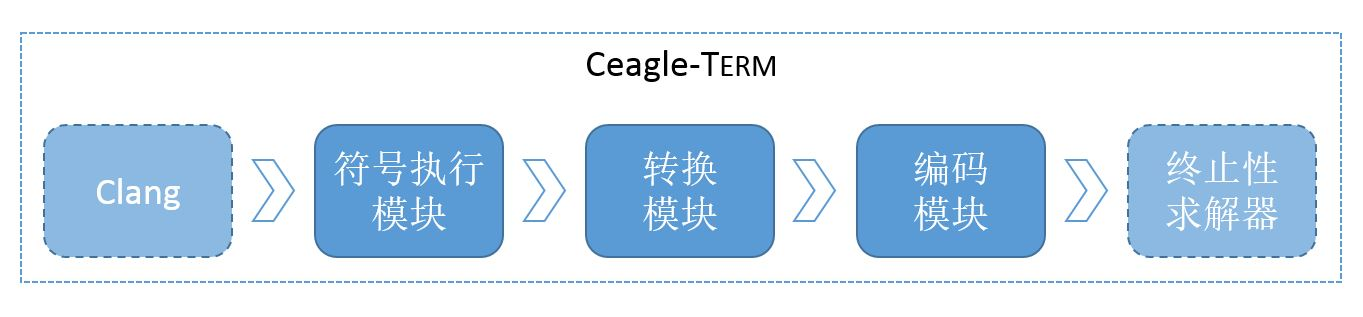
\includegraphics[width=\textwidth]{Ceagle-Termination.jpg}
\caption{\CTerm 组成}
\label{f:Ceagle-Termination}
\end{figure}

如图~\ref{f:Ceagle-Termination} 所示, \CTerm 主要由三部分构成:符号执行模块,转换模块和编码模块。前端接入第三方工具 Clang,将待验证的 C 程序编译成为 LLVM IR 程序。符号执行模块接受 LLVM IR 代码输入,生成对应的符号执行图。符号执行图经过转换模块后,输出整数变迁系统。该变迁系统经过编码模块的编码,生成适合后端重写模型终止性求解器的整数重写模型。后端接入第三方终止性求解器(目前支持开源求解器 \verb|KITTeL|~\cite{DBLP:conf/rta/FalkeKS11}),求解输出终止性验证结果。


\begin{algorithm}[htbp]
  \KwIn{$G$:只包含初始状态顶点的符号执行图}
  \KwIn{$path$:存放顶点的栈结构,初始状态只包含初始顶点}
  \KwOut{$G$:构建完成的符号执行图}

  \While{ $path$ 非空 }{
    $v = peek(path)$\;
    \uIf{$v.visited == false$}{
      
      \If(\tcp*[h]{如果 $v$ 是结束状态}){$v == END$} {
        $v.visited = true$; \qquad $path.pop()$\;
        continue\;
      }

      %\tcp{decide whether we should generalize}
      在 $path$ 中寻找程序位置与 $v$ 相同的顶点,组成列表 $list_v$ \;
      %$list = path.findSamePC(v)$\;
      $should = false$ \tcp*{判断是否应该进行抽象}

      \ForEach{$u\in list_v$}{
        \If{ $u$ 和 $v$ 满足应该抽象的判断条件 }{
            %$u.domain() == v.domain()$ \\
            %$\land$ $v$ has an incoming evaluation edge \\
            %$\land$ $u$ has no incoming refinement edge}{
          $should = true$; \qquad $target = u$\;
          break\;
        }
      }

      %\tcp{Now we know what we should do}
      \uIf{should}{
        %\tcc{Do generalization}
        %perform Algorithm~\ref{a:generalization}\;
        应用算法~\ref{alg:abstraction} 进行抽象\;
      } \Else {
        %\tcc{Do evaluation}
        %perform Algorithm~\ref{a:evaluation}\;
        应用算法~\ref{alg:evaluation} 进行符号执行\;
      }
    } \Else(\tcp*[h]{ $v$ 已被访问过}) {
      在 $G$ 中寻找一个未被访问的 $v$ 的后继顶点 $w$\;
      \uIf{ $w$ 不存在} {
        $pop(path)$\tcp*{将 $v$ 从栈中取出}
      } \Else {
        $push(w,path)$\;
      }
    }
  }
\caption{构建符号执行图}
\label{alg:seg}
\end{algorithm}

\begin{algorithm}[htbp]
\KwIn{$G$:正在构建的符号执行图 }
\KwIn{$v$:正在访问的顶点 }
\KwIn{$target$:$v$ 的抽象目标顶点 } 
\KwIn{$path$:当前搜索路径}
\KwOut{$G$, $path$}
  \uIf{ 状态 $target$ 是 $v$ 的抽象 }{
    $v.visited = true$\;
    %$G.add\_edge(v,genTarget,generalization)$\;
    在 $G$ 中添加从 $v$ 到 $target$ 的一条抽象类型的边\;
    $pop(path)$\tcp*{将 $v$ 从栈中取出}
  } \Else(\tcp*[h]{ 需要计算 $v$ 和 $target$ 的抽象 }) { 
    %$path.popupto(genTarget)$\;
    对 $path$ 进行出栈操作,直到 $target$ 成为栈顶元素\;
    %$G.removeChild(genTarget)$\;
    在 $G$ 中删除 $target$ 的后继顶点\;
    %$c = merge(v, genTarget)$\;
    %$G.add\_vertex(c)$\;
    计算 $v$ 和 $target$ 的抽象状态 $c$,并将其加入 $G$\;

    \uIf{ 如果 $path$ 中只含 $target$ 一个元素 } {
      %$G.add\_edge(genTarget,c,generalization)$\;
      在 $G$ 中添加从 $target$ 到 $c$ 的一条抽象类型的边\;
      $push(c,path)$\;
    } \Else {
      $pop(path)$\tcp*{将 $target$ 从栈中取出}
      $p = peek(path)$\;
      \uIf{ 在 $G$ 中存在从 $p$ 到 $target$ 的抽象类型的边 }{
        从 $G$ 中删除顶点 $target$ 及其边\;
        在 $G$ 中添加从 $p$ 到 $c$ 的一条抽象类型的边\;
        $push(c,path)$\;
      } \Else {
        在 $G$ 中添加从 $target$ 到 $c$ 的一条抽象类型的边\;
        $push(target,path)$\;
        $push(c,path)$\;
      }
    }
  }
\caption{状态抽象}
\label{alg:abstraction}
\end{algorithm}

\begin{algorithm}[htbp]
\KwIn{$G$:正在构建的符号执行图 }
\KwIn{$v$:正在访问的顶点 }
\KwIn{$path$:当前搜索路径}
\KwOut{$G$, $path$}
  $v.visited = true$\;
  %$stateList = v.evaluate()$\;
  对状态 $v$ 应用除抽象外的符号执行规则,获得新状态列表 $list_{new}$\;
  \uIf(\tcp*[h]{没有对 $v$ 应用精化规则 }){$size(list_{new}) == 1$ } {
    $w = list_{new}[0]$\;
    在 $G$ 中添加顶点 $w$ 以及从 $v$ 到 $w$ 的一条求值类型的边\;
    $push(w,path)$\;
  } \Else(\tcp*[h]{ 精化规则被应用,产生2个新状态 }) {
    $w_1 = list_{new}[0]$\;
    $w_2 = list_{new}[1]$\;
    在 $G$ 中添加顶点 $w_1$ 以及从 $v$ 到 $w_1$ 的一条求值类型的边\;
    在 $G$ 中添加顶点 $w_2$ 以及从 $v$ 到 $w_2$ 的一条求值类型的边\;
    $push(w_1,path)$\;
  }
\caption{求值与精化}
\label{alg:evaluation}
\end{algorithm}

\CTerm 的核心模块为符号执行模块,它涉及到对每一个抽象程序状态的符号执行、计算两个状态的抽象状态、以及对整个符号执行图进行构建。对状态的符号执行与抽象计算已经在小节\ref{ss:seg} 进行介绍,在此不再赘述。下面给出构建符号执行图的核心算法,见算法~\ref{alg:seg}。 

\subsection{性能评估} 
\todo{需要等到工具原型开发完成}
 
\todo{与 AProVE 、\texttt{KITTeL}、Ctrl 进行比较} 

\subsection{可扩展性}

由于 \CTerm 的核心模块——符号执行模块是针对 LLVM IR 实现的,得益于 LLVM 一般化的框架及丰富的工具集,通过接入不同的前端,\CTerm 可以支持更多类型的程序终止性验证。比如利用 GCC 搭配 DragonEgg~\cite{dragonegg} 作为前端,则可以实现对 Ada 语言~\cite{DBLP:journals/computer/WolfeBSTW81} 和 Fortran 语言~\cite{DBLP:books/sp/ChiversS15} 程序的终止性验证。

从后端的角度看,由于 \CTerm 输出的模型及模型格式由编码模块决定,因此通过对编码模块进行扩展,可以实现后端对更多重写模型终止性求解器的支持,比如 Ctrl~\cite{DBLP:conf/lpar/Kop015} 和 \TTT~\cite{DBLP:conf/rta/KorpSZM09}。 


\section{本章小结}

整数重写模型是规范化条件重写模型的一种特例。基于整数重写模型和符号执行图,我们开发了针对 C 语言程序终止性的自动验证工具 \CTerm。该工具接受 C 语言程序输入,并自动对其进行模型转换与终止性求解,不需要人工参与。

\todo{评价其表现}
